\documentclass[11pt]{beamer}

% Theme / appearance
\usetheme{Madrid}
\usecolortheme{seahorse}
\setbeamertemplate{navigation symbols}{}
\setbeamertemplate{caption}[numbered]

% Encoding and language
\usepackage[utf8]{inputenc}
\usepackage[T1]{fontenc}
\usepackage[ngerman,english]{babel} % English main, German available

% Math and symbols
\usepackage{amsmath,amssymb,amsthm,mathtools}
\usepackage{bm}
\usepackage{siunitx}

% Graphics and tikz
\usepackage{graphicx}
\usepackage{tikz}
\usepackage{pgfplots}
\pgfplotsset{compat=1.18}

% Micro typography
\usepackage{microtype}

% Colors, links
\usepackage{xcolor}
% \usepackage[hidelinks]{hyperref}

% Useful shortcuts
\newcommand{\logit}{\operatorname{logit}}
\newcommand{\sigmoid}{\sigma}
\newcommand{\E}{\mathbb{E}}
\newcommand{\Var}{\operatorname{Var}}

% Title data — anpassen nach Bedarf
\title[Poisson \(\to\) Polya–Gamma]{From Poisson to Polya–Gamma in Spatial Models}
\author[T. Luhdo]{Toni Luhdo}
\institute[UP]{University of Potsdam}
\date[Habana 2026]{Habana Encuentro, 2026}

% Optional: Outline before sections
\AtBeginSection[]{
  \begin{frame}{Outline}
    \tableofcontents[currentsection]
  \end{frame}
}

\begin{document}

\titlepage

\section{Motivation: Earthquake Intensity Field}

\begin{frame}{Earthquake Events as Point Data}
We observe earthquake epicenters as spatial point data.

\begin{center}
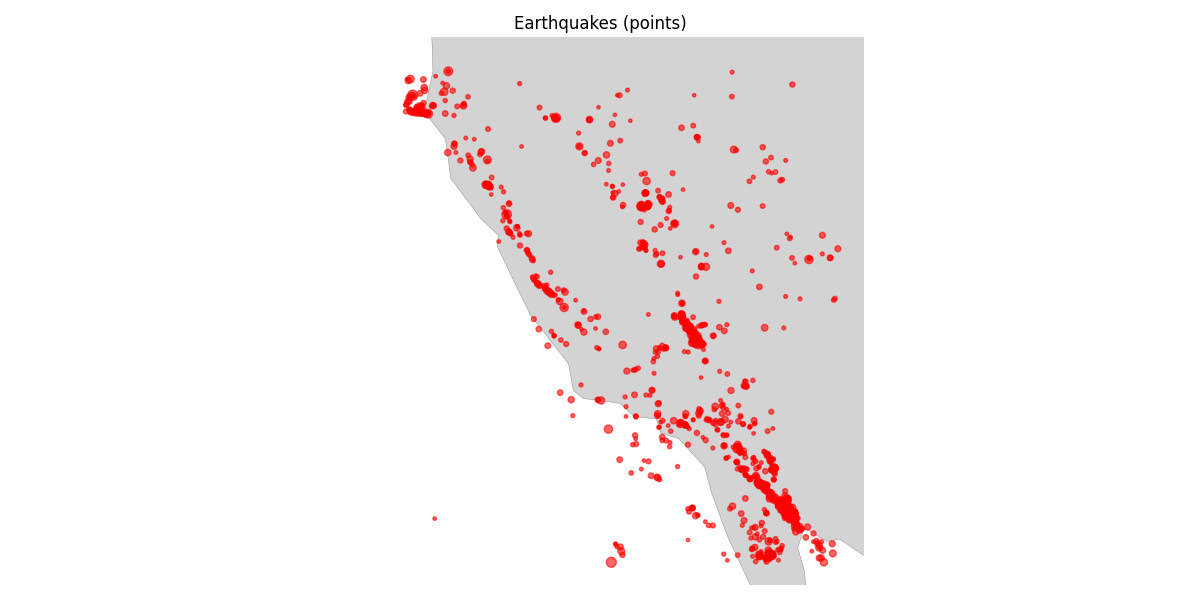
\includegraphics[width=0.8\textwidth]{figures/earthquakes_points.png}
\end{center}

Goal:
\begin{itemize}
\item Estimate a smooth spatial intensity field.
\item Identify high-risk regions.
\item Quantify uncertainty.
\end{itemize}
\end{frame}

\begin{frame}{From Points to Counts}
After gridding the region:

\[
n_i = \text{number of earthquakes in cell } i
\]

\begin{center}

\includegraphics[width=0.95\textwidth]{figures/Figure_1.png}
\end{center}

We now model:
\[
n_i \sim \text{Poisson}(\lambda_i)
\]
\end{frame}

\section{Poisson Model with Logistic Structure}

\begin{frame}{Basic Poisson Model}
\[
n_i \sim \text{Poisson}(\lambda_i)
\]

Instead of modeling $\lambda_i$ directly,
we introduce a latent field $f_i$:

\[
\lambda_i = \lambda \, \sigma(f_i),
\quad
\sigma(f) = \frac{1}{1+e^{-f}}
\]

\begin{itemize}
\item $f_i$ captures spatial structure
\item $\lambda$ is global intensity
\item $\sigma$ keeps rates bounded and stable
\end{itemize}
\end{frame}


\section{Likelihood Derivation}

\begin{frame}{Poisson Likelihood}
\[
p(n_i \mid f_i,\lambda)
=
\frac{(\lambda \sigma(f_i))^{n_i}}{n_i!}
\exp(-\lambda \sigma(f_i))
\]

Log-likelihood:
\[
\ell(f)
=
\sum_i
\left(
n_i \log \sigma(f_i)
-
\lambda \sigma(f_i)
\right)
\]


Problem:
\begin{itemize}
\item Non-quadratic in $f$
\item No conjugacy with Gaussian prior
\end{itemize}
\end{frame}

%-----------------------------------------------------------
\begin{frame}{Posterior: What Do We Want?}

Model:

\[
n_i \sim \text{Poisson}(\lambda \sigma(f_i)),
\qquad
\sigma(f)=\frac{1}{1+e^{-f}}
\]

Prior on latent field:

\[
f \sim \mathcal{N}(\mu,\Sigma)
\]

Posterior target:

\[
p(f \mid n) \propto p(n \mid f)\, p(f)
\]

Difficulty:

\[
\sigma(f) \quad \Rightarrow \quad
\text{non–quadratic log-likelihood}
\]

Therefore Gaussian conjugacy is lost.

\end{frame}

%-----------------------------------------------------------
\begin{frame}{Log-Likelihood Structure}

From the Poisson model:

\[
p(n_i \mid f_i,\lambda)
=
\frac{(\lambda \sigma(f_i))^{n_i}}{n_i!}
\exp(-\lambda \sigma(f_i))
\]

Log-likelihood:

\[
\ell(f)
=
\sum_i
\left(
n_i \log\sigma(f_i)
-
\lambda\sigma(f_i)
\right)
\]

The problematic terms are

\[
n_i\log\sigma(f_i), 
\qquad
-\lambda\sigma(f_i)
\]

which prevent a Gaussian posterior.

\end{frame}

%-----------------------------------------------------------
\begin{frame}{Trick 1: Poisson Splitting}

We rewrite the exponential term:

\[
e^{-\lambda\sigma(f_i)}
=
e^{-\lambda(1-\sigma(-f_i))}
=
e^{-\lambda}\,e^{\lambda\sigma(-f_i)}
\]

Using the Poisson series expansion:

\[
e^{\lambda\sigma(-f_i)}
=
\sum_{k_i=0}^{\infty}
\frac{(\lambda\sigma(-f_i))^{k_i}}{k_i!}
\]

This suggests introducing latent counts.

\end{frame}

%-----------------------------------------------------------
\begin{frame}{Latent Negative Counts}

Introduce auxiliary variables:

\[
k_i \mid f_i
\sim
\text{Poisson}(\lambda\sigma(-f_i))
=
\text{Poisson}\left(\frac{\lambda}{1+e^{f_i}}\right)
\]

Augmented likelihood:

\[
p(n_i,k_i \mid f_i)
\propto
(\lambda\sigma(f_i))^{n_i}
(\lambda\sigma(-f_i))^{k_i}
\]

Using

\[
\sigma(f)=\frac{e^f}{1+e^f},
\qquad
\sigma(-f)=\frac{1}{1+e^f}
\]

we obtain a logistic form.

\end{frame}

%-----------------------------------------------------------
\begin{frame}{Emergence of Logistic Structure}

After substitution:

\[
p(n_i,k_i \mid f_i)
\propto
\frac{e^{n_i f_i}}{(1+e^{f_i})^{n_i+k_i}}
\]

Define

\[
b_i = n_i + k_i
\]

Then

\[
p(n_i,k_i \mid f_i)
\propto
\frac{e^{n_i f_i}}{(1+e^{f_i})^{b_i}}
\]

This is exactly the form required for
Pólya–Gamma augmentation.

\end{frame}

%-----------------------------------------------------------
\begin{frame}{Trick 2: Pólya--Gamma Identity}

The Polson--Scott--Windle identity states:

\[
\frac{e^{\kappa f}}{(1+e^f)^b}
=
2^{-b}
\int_0^\infty
\exp\!\left(-\frac{\omega f^2}{2} + \kappa f\right)
p(\omega \mid b,0)
d\omega
\]

with

\[
\kappa_i = n_i - \frac{b_i}{2}
\]

This converts the logistic likelihood
into a Gaussian kernel.

\end{frame}

%-----------------------------------------------------------
\begin{frame}{Tilted Pólya--Gamma Variables}

Introducing latent variables:

\[
\omega_i \mid f_i,b_i
\sim
\text{PG}(b_i,f_i)
\]

Conditional likelihood:

\[
\log p(f_i \mid \omega_i)
=
-\frac12 \omega_i f_i^2
+ 
\kappa_i f_i
+
\text{const}
\]

The likelihood becomes quadratic in $f_i$.

\end{frame}

%-----------------------------------------------------------
\begin{frame}{Combining with the Gaussian Prior}

Prior:

\[
f \sim \mathcal{N}(\mu,\Sigma)
\]

Log prior:

\[
\log p(f)
=
-\frac12 (f-\mu)^\top
\Sigma^{-1}
(f-\mu)
\]

Expand:

\[
(f-\mu)^\top\Sigma^{-1}(f-\mu)
=
f^\top\Sigma^{-1}f
-2f^\top\Sigma^{-1}\mu
+
\mu^\top\Sigma^{-1}\mu
\]

\end{frame}

%-----------------------------------------------------------
\begin{frame}{Log Posterior Kernel}

Combining likelihood and prior:

\[
\log p(f\mid n,k,\omega)
=
-\frac12 f^\top(\Sigma^{-1}+\Omega)f
+
f^\top(\Sigma^{-1}\mu+\kappa)
+
c
\]

where

\[
\Omega = \text{diag}(\omega_1,\dots,\omega_n)
\]

This has the standard quadratic form

\[
-\frac12 f^\top Q f + f^\top h
\]

\end{frame}

%-----------------------------------------------------------
\begin{frame}{Identify the Gaussian Posterior}

Define

\[
Q = \Sigma^{-1}+\Omega,
\qquad
h = \Sigma^{-1}\mu+\kappa
\]

Gradient of log posterior:

\[
\nabla_f \log p
=
-Qf + h
\]

Setting the gradient to zero:

\[
Qm = h
\]

Therefore

\[
f \mid \omega,n,k
\sim
\mathcal{N}(m,Q^{-1})
\]

\end{frame}

%-----------------------------------------------------------
\begin{frame}{Sampling the Latent Field}

In practice we avoid computing $Q^{-1}$.

Instead:

\begin{itemize}
\item Compute Cholesky factorization
\[
Q = LL^\top
\]

\item Solve
\[
L^\top x = z, \quad z\sim \mathcal{N}(0,I)
\]

\item Sample
\[
f = m + x
\]
\end{itemize}

This step scales well for high-dimensional
spatial fields.

\end{frame}


% \section{Poisson Splitting Trick}

\begin{frame}{Poisson Splitting Trick - Introduce Latent Counts}
Define additional latent variables:

\[
k_i \sim \text{Poisson}(\lambda(1-\sigma(f_i)))
\]

Since

\[
\sigma(f) = \frac{e^f}{1+e^f}
\quad
1-\sigma(f)=\frac{1}{1+e^f}
\]

we obtain:

\[
p(n_i,k_i \mid f_i)
\propto
\frac{e^{n_i f_i}}{(1+e^{f_i})^{n_i+k_i}}
\]

Define:
\[
b_i = n_i + k_i
\]
\end{frame}


\section{Pólya--Gamma Identity}

\begin{frame}{Key Identity}
Polson–Scott–Windle identity:

\[
\frac{e^{\kappa f}}{(1+e^f)^b}
=
2^{-b}
\int_0^\infty
e^{-\frac{\omega f^2}{2}}
p(\omega \mid b,0)
\, d\omega
\]

with

\[
\kappa = n_i - \frac{b_i}{2}
\]

Conditional representation:

\[
\omega_i \mid f_i,b_i
\sim
\text{PG}(b_i,f_i)
\]
\end{frame}


\begin{frame}{Why This Is Powerful}
After introducing $\omega_i$:

\[
\log p(f_i \mid \omega_i)
=
-\frac12 \omega_i f_i^2
+
\kappa_i f_i
+
\text{const}
\]

This is quadratic in $f_i$.

\bigskip

Quadratic $\implies$ Gaussian conditional posterior.
\end{frame}


\section{Gibbs Sampler}

\begin{frame}{Full Conditional Updates}

For each iteration:

\textbf{1) Latent counts}
\[
k_i \sim \text{Poisson}\left(\frac{\lambda}{1+e^{f_i}}\right)
\]

\textbf{2) Pólya–Gamma}
\[
\omega_i \sim \text{PG}(b_i,f_i)
\]

\textbf{3) Latent field}
\[
f \sim \mathcal{N}(m,Q^{-1})
\]

where

\[
Q = \Sigma^{-1} + \Omega
\]
\end{frame}

\begin{frame}{Why This Works So Well}
\begin{itemize}
\item No Metropolis tuning
\item Exact conditional updates
\item Fully Gaussian step for high-dimensional $f$
\item Works beautifully with sparse precision matrices
\end{itemize}
\end{frame}


\section{Application: Earthquake Data}

\begin{frame}{Earthquake Events as Point Data}
We observe earthquake epicenters as spatial point data.

\begin{center}
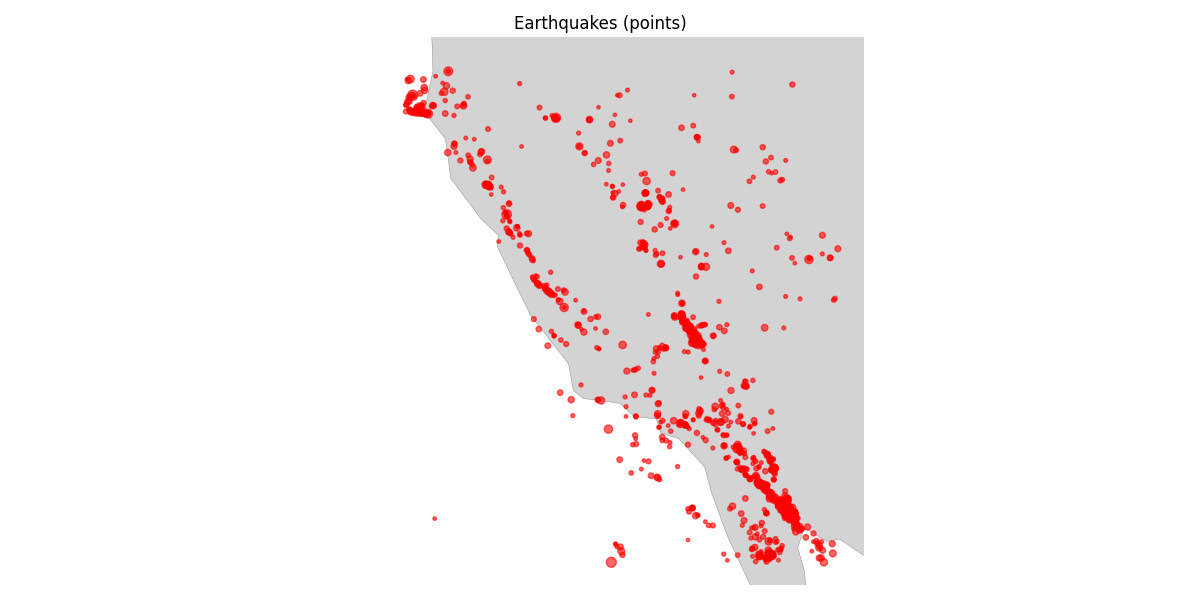
\includegraphics[width=1.1\textwidth]{figures/earthquakes_points.png}
\end{center}

\end{frame}

\begin{frame}{Observed Counts}
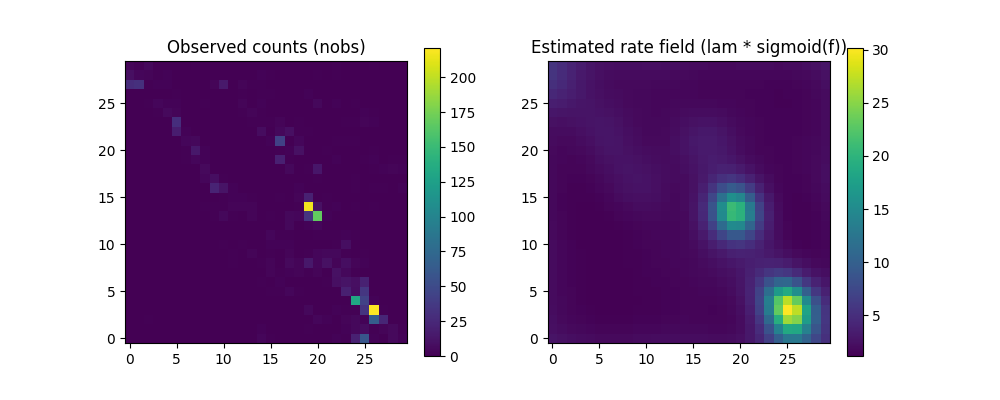
\includegraphics[width=1.1\textwidth]{figures/figure_1.png}
\end{frame}

\begin{frame}{Observed Counts log scale}
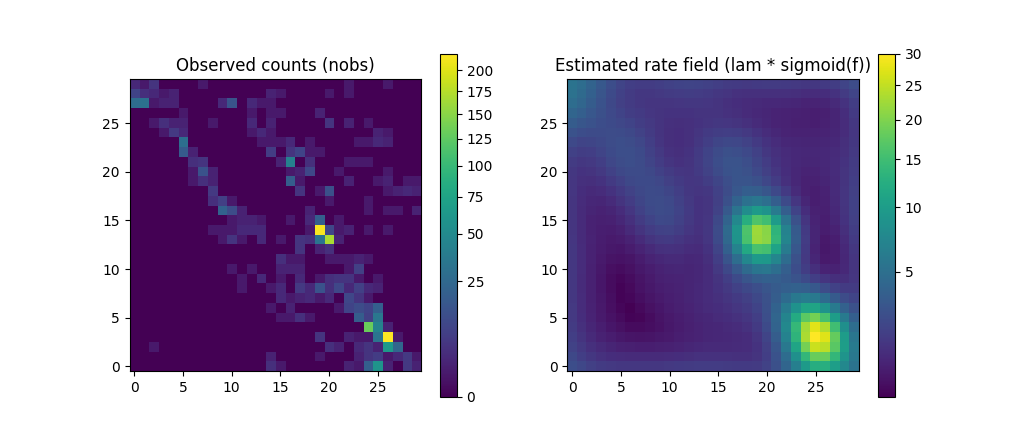
\includegraphics[width=1.1\textwidth]{figures/figure_2.png}
\end{frame}

\begin{frame}{Takeaways}
\begin{itemize}
\item Poisson model with logistic link
\item Poisson splitting introduces logistic structure
\item Pólya–Gamma augmentation makes inference Gaussian
\item Efficient Gibbs sampling for spatial fields
\item Application: Earthquake intensity estimation
\end{itemize}
\end{frame}

\begin{frame}{References}
  \scriptsize
\begin{itemize}
\item Polson, N. G., Scott, J. G., & Windle, J. (2013). Bayesian inference for logistic models using Pólya–Gamma latent variables. \textit{Journal of the American Statistical Association}, 108(504), 1339-1349.
\item Linderman, S., Johnson, M., & Adams, R. P. (2015). Dependent multinomial models made easy: Stick-breaking with the Pólya–Gamma augmentation. In \textit{International Conference on Machine Learning} (pp. 1114-1123).
\item Zhou, M., & Carin, L. (2015). Negative binomial process count and mixture modeling. \textit{IEEE Transactions on Pattern Analysis and Machine Intelligence}, 37(2), 307-320.
\end{itemize}
\end{frame}

\begin{frame}{Thank you!}
  \begin{center}
    \Large Thank you for your attention!\\
      \vspace{1cm}
  Questions?
  \end{center}
\end{frame}
\section*{Appendix}

\begin{frame}{Estimated Rate Field}
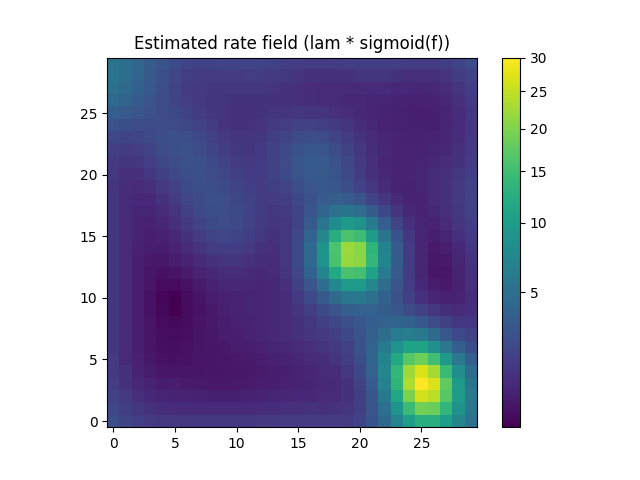
\includegraphics[width=0.9\textwidth]{figures/estimated_rate_field.png}

Posterior mean:
\[
\hat{\lambda}_i = \lambda \, \sigma(f_i)
\]
\end{frame}


\end{document}